%%%%%%%%%%%%%%%%%%%%%%%%%%%%%%%%%%%%%%%%%%%%%%%%%%%%%%%%%%%%%%%%%%%%%%%%
% Golden Sacra - Memoria
% Escuela Politécnica Superior de la Universidad de Alicante
% Realizado por: Ángel Jesús Terol Martínez
% Contacto: jtm37@alu.ua.es
%%%%%%%%%%%%%%%%%%%%%%%%%%%%%%%%%%%%%%%%%%%%%%%%%%%%%%%%%%%%%%%%%%%%%%%%

\chapter{Resumen}
\label{resumen}
\textbf{Golden Sacra} es un juego de aventuras, RPG o nethack, para la consola Game Boy, el cual recibe influencia de títulos como \textbf{Pokémon Mundo Misterioso} o \textbf{Shiren the Wanderer}. \\ \\
El juego funciona por \textbf{turnos}: habrá un turno para la acción del jugador y otro para cada enemigo. Cada vez que ataquemos, nos movamos o usemos un objeto, nuestro turno se consumirá. El \textbf{gameplay} se desarrolla principalmente en el \textbf{interior de una mazmorra}, compuesta por \textbf{distintos pisos} a las cuales podremos acceder gracias a unas escaleras. \\ \\
Estará realizado completamente en lenguaje ensamblador o Z80, y en este documento se recogerá todo el proceso de diseño y desarrollo, junto a las herramientas o frameworks utilizados para ello.
{\let\clearpage\relax\chapter*{Abstract}}

\textbf{Golden Sacra} is an adventure, RPG or nethack game, for the original Game Boy, which is influenced by titles such as \textbf{Pokémon Mystery Dungeon} or \textbf{Shiren the Wanderer}.
\\ \\
The game works by \textbf{turns}: there will be a turn for player action and another for each enemy. Each time we attack, move or use an object, our turn will be consumed. The \textbf{gameplay} is mainly developed inside a dungeon, composed of \textbf{different floors} that we can access thanks to some stairs that can be found in each one.
\\ \\
It will be done entirely in assembly language or Z80, and this document will cover the entire design and development process, along with the tools or frameworks used for it.
\cleardoublepage

\chapter{Objetivos}
\label{objetivos}

A día de hoy es difícil encontrar desarrolladores de videojuegos que se preocupen realmente de \textbf{qué está ocurriendo en la máquina} con cada instrucción que escriben gracias a la facilidad que ofrecen los entornos modernos actuales y la cantidad de información que se puede encontrar en las redes.
Un \textbf{ingeniero} debe ser capaz en todo momento de \textbf{resolver los problemas} que se le planteen por si mismo y no basarse en buscar la solución de alguien anónimo.\\ \\
Las arquitecturas de las máquinas actuales son \textbf{complejas y muy potentes} para que una persona les pueda sacar todo el potencial en un corto período de tiempo. Por ello, lo ideal es empezar por una consola más antigua como punto de partida, como lo puede ser la propia \textbf{Game Boy}.\\ \\
La razón de escogerla como la consola sobre la que desarrollar este proyecto ha sido \textbf{subjetiva} debido al afecto que le tengo. Perfectamente podría haber escogido cualquier otra como la \textit{NES} o la \textit{Master System}. Por otro lado, con la documentación de esta memoria pretendo \textbf{ser de ayuda para más personas} que se propongan en un futuro realizar un juego para dicha consola.\\ \\
A grandes rasgos, los objetivos serían los siguientes:\\
\begin{itemize}
	\item \textbf{Analizar la Nintendo Game Boy y entender sus capacidades y limitaciones.}
	\item \textbf{Analizar librerías y frameworks existentes.}
	\item \textbf{Aprender programación en ensamblador.}
	\item \textbf{Comprender el funcionamiento del hardware.}
	\item \textbf{Diseñar y desarrollar un videojuego completo.}
\end{itemize}

Objetivos secundarios:

\begin{itemize}
	\item \textbf{Realizar una publicación física del videojuego.}
	\item \textbf{Distribuir el videojuego.}
\end{itemize}

\cleardoublepage

\chapter{Terminología}
\label{terminologia}
A lo largo del documento se van a utilizar varias nomenclaturas para hacer la lectura más sencilla:
\begin{itemize}
	\item \textbf{GB:} Game Boy.
    \item \textbf{GBC:} Game Boy Color.
    \item \textbf{SGB:} Super Game Boy.
	\item \textbf{RGBDS:} Rednex Game Boy Development System. Ensamblador y enlazador para la Game Boy y Game Boy Color.
	\item \textbf{Bit:} Unidad mínima de información empleada en informática.
	\item \textbf{Byte:} Unidad de información equivalente a 8 bits.
	\item \textbf{CPU:} Central Processing Unit. Hardware que interpreta las instrucciones del programa.
	\item \textbf{GPU:} Graphics Processing Unit. Hardware dedicado al procesamiento de gráficos.
	\item \textbf{RAM:} Random Access Memory. Memoria de trabajo donde almacenamos nuestras variables.
    \item \textbf{ROM:} Read Only Memory. Zona de memoria donde se almacena el código del programa.
	\item \textbf{VRAM:} Video RAM. Zona de memoria utilizada por el controlador gráfico para representar información de manera visual por pantalla.
	\item \textbf{HRAM:} High RAM. Zona de memoria accesible en el proceso DMA. 
    \item \textbf{DMA:} Direct Memory Access. Característica de ciertos sistemas informáticos que permite acceder a RAM a un subsistema, indepentientemente de la CPU.
    \item \textbf{OAM:} Object Attribute Memory. Espacio de memoria en el que se almacenan los atributos de los sprites.
    \item \textbf{Sprite:} Elemento visual activo en pantalla.
	\item \textbf{Tile:} Conjunto de pixeles de tamaño 8x8.
	\item \textbf{GBTD:} Game Boy Tile Designer. Programa para diseñar tiles.
	\item \textbf{GBMB:} Game Boy Map Builder. Programa para construir tilemaps.
	\item \textbf{BGB:} Emulador de GB, GBC y SGB.
	\item \textbf{NO\$GMB:} Equivalente al BGB, pero obsoleto.
\end{itemize}

\cleardoublepage

\chapter{Metodología y Planificación}
\label{planificacion}

El \textbf{tipo de metodologías} aplicadas a la hora de planificar el proyecto son las \textbf{ágiles}. Si bien este tipo de metodologías suelen aplicarse a proyectos en grupo, es importante tener calculados los tiempos que se debe emplear a cada tarea con el fin de \textbf{obtener el mejor resultado en el plazo de tiempo correspondiente}.
\\ \\
\textbf{El proyecto está dividido en distintas etapas/iteraciones}, sobre las cuales se van aprendiendo y poniendo en práctica nuevos aspectos respectivos al proyecto. Además, \textbf{al finalizar cada iteración}, se hace una \textbf{revisión del mismo} para ver en detalle que necesita mejorar o arreglar, e intentar de esta manera perder el mínimo tiempo posible. \textbf{Las tareas cambian y se modifican constantemente} a lo largo del desarrollo, debido a que, al partir de 0, los conocimientos aumentan progresivamente. Esto implica que lo que al principio parecía estar bien implementado al final hay que, en la mayoría de casos, rehacerlo.
\\ \\
El proyecto se ha dividido en las siguientes etapas/iteraciones:

\begin{itemize}
	\item \textbf{Diseño}
	
	Lo principal es tener en mente lo que se quiere llevar a cabo. Se hará un pequeño análisis de los distintos juegos y géneros de los que dispone el catálogo de la consola, así como la posible dificultad técnica que tengan, a partir del cual obtener una idea sólida del proyecto a realizar. Realizar un pequeño GDD también nos ayudará a que estas ideas no se modifiquen o pierdan con el paso del tiempo.

	\item \textbf{Aprendizaje}
	
	Esta iteración se utilizará exclusivamente para analizar en profundidad las limitaciones de la consola, así como realizar distintas pruebas que puedan llegar a servir como base a la hora de dar comienzo con el desarrollo.
	
	\item \textbf{Desarrollo}
	
	La etapa principal del proyecto en la que vamos a invertir más tiempo. Se irá desarrollando el producto y, al mismo tiempo, realizando la documentación pertinente.
	
	\item \textbf{Revisión y Maquetación}
	
	Esta última etapa servirá para revisar tanto el producto como la documentación de la memoria y su maquetación. También se utilizará para arreglar posibles errores del videojuego o realizar pequeñas mejoras.
	
\end{itemize}	

\clearpage

Las \textbf{herramientas principales} que se van a utilizar son \textbf{Trello y Toggl}. Además, como herramienta de \textbf{control de versiones}, se va a hacer uso de \textbf{Git}.
\\ \\
En Trello se ha creado una tabla con la que poder visualizar de manera sencilla qué tareas están pendientes de realizar, tanto del producto como de la memoria. Todas estas tareas pasarán a la fase de revisión y, una vez dado el visto bueno, terminarán en el estado de finalizado.

\begin{figure}[h]
\centering
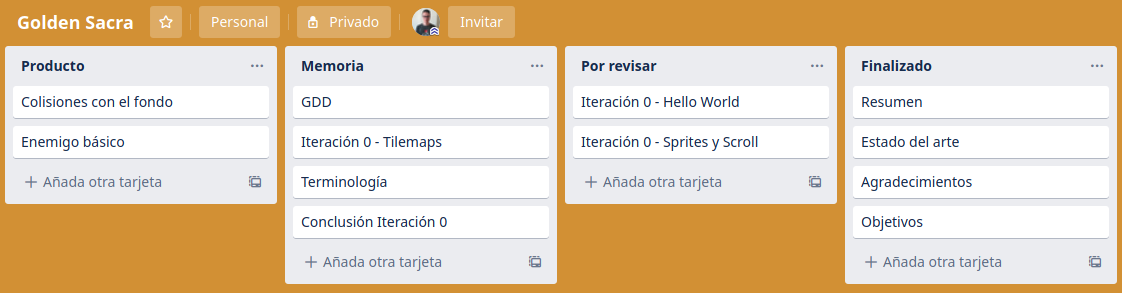
\includegraphics[width=1\textwidth]{include/images/gdd/trello.png}
\caption{Tabla Trello - Iteración 0}
\label{figure:trello}
\end{figure}
	
\section{Mínimo Producto Viable}

Lo normal en todo proyecto es que ocurran imprevistos que hagan al programador perder más tiempo en una tarea o incluso paralizar por completo el proyecto. Además, esto se junta con el hecho de que aquí no hay nadie que pueda ocupar nuestro puesto mientras ese problema se soluciona. Por esta razón, es importante tener en mente un \textbf{producto mínimo viable}, con el cual obtener un producto jugable de inicio a fin en el tiempo disponible.
\\ \\
En nuestro caso, el producto mínimo sería \textbf{una mazmorra}, \textbf{enemigos} que te puedan matar, \textbf{objetos} que usar, \textbf{y las mecánicas básicas} del jugador.
\\ \\
Más que producto se le debería de calificar de \textbf{prototipo}, pero no deja de ser un \textbf{proyecto cerrado y terminado} con el que la gente pueda jugar.
	
\cleardoublepage






